\section{Grafici ed immagini}

\begin{figure}[h]
	\centering
	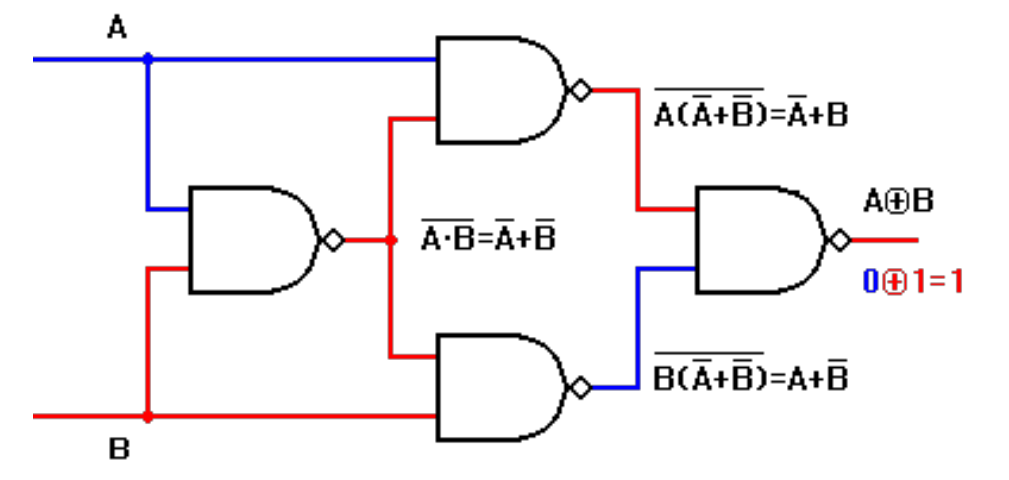
\includegraphics[scale=0.4]{xor_circuito.png}
	\caption{Circuito XOR}
	\label{f:xor_circuito}
\end{figure}

\begin{figure}[h]
	\centering
	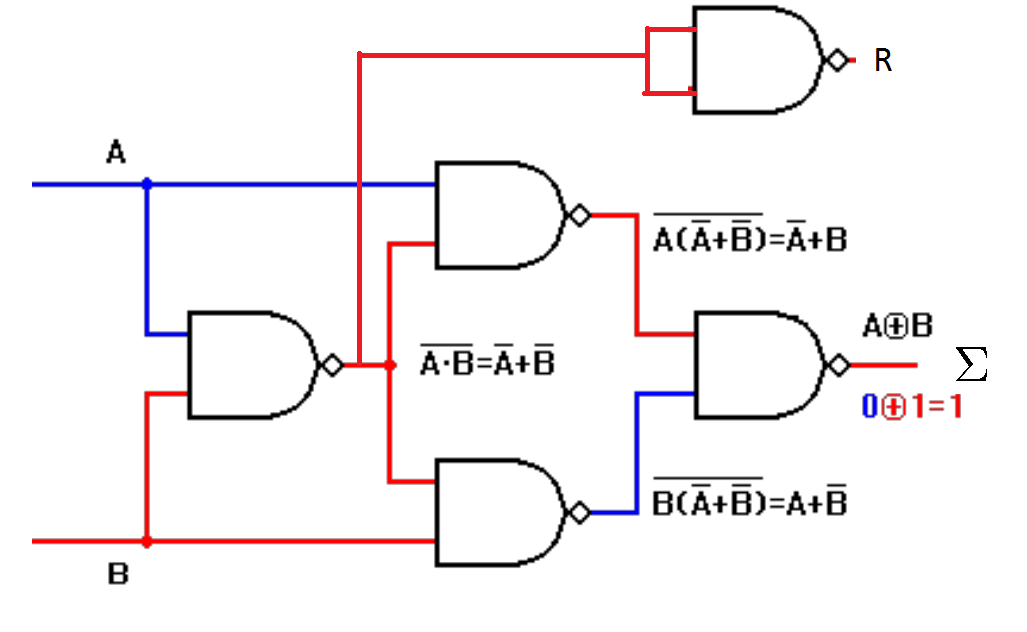
\includegraphics[scale=0.4]{sommatore_circuito.png}
	\caption{Circuito sommatore}
	\label{f:sommatore_circuito}
\end{figure}

\begin{figure}[h]
	\centering
	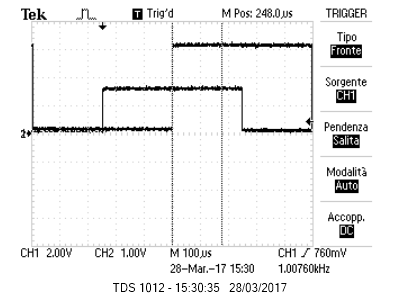
\includegraphics[scale=0.6]{ingresso.png}
	\caption{Segnali in ingresso; entrambi hanno valore alto di $\sim$ 3.2V.  il segnale visualizzato con la scala di CH1 è Y1, mentre quello in CH2 è Y2.}
	\label{f:ingressi}
\end{figure}

\begin{figure}[h]
	\centering
	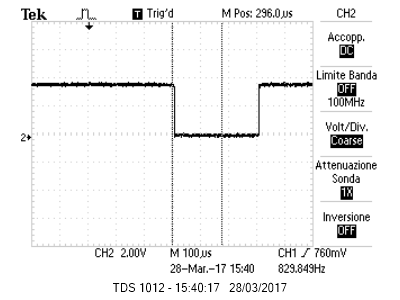
\includegraphics[scale=0.6]{nand.png}
	\caption{Uscita del circuito NAND }
	\label{f:NAND}
\end{figure}

\begin{figure}[h]
	\centering
	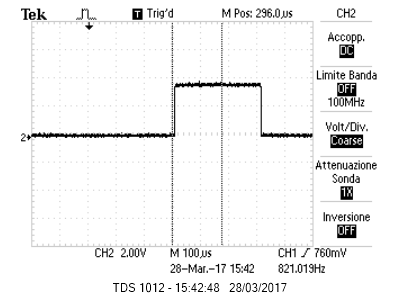
\includegraphics[scale=0.6]{and.png}
	\caption{Uscite del circuito AND.}
	\label{f:AND}
\end{figure}

\begin{figure}[h]
	\centering
	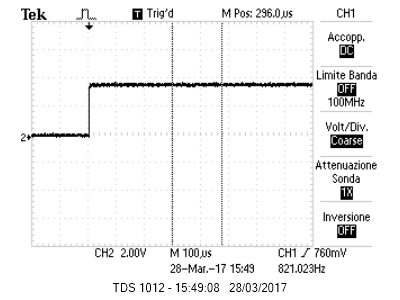
\includegraphics[scale=0.6]{or.png}
	\caption{Uscita del circuito OR}
	\label{f:OR}
\end{figure}

\begin{figure}[h]
	\centering
	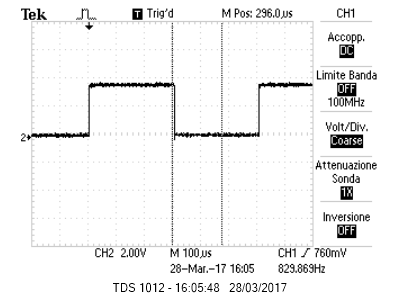
\includegraphics[scale=0.6]{xor.png}
	\caption{Uscita del circuito XOR}
	\label{f:XOR}
\end{figure}

\begin{figure}[h]
	\centering
	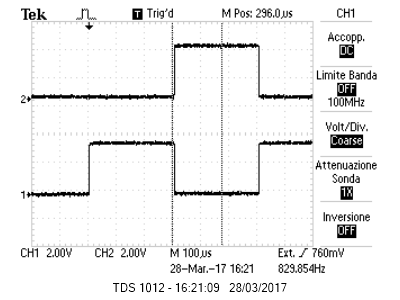
\includegraphics[scale=0.6]{sommatore.png}
	\caption{Uscite del circuito sommatore (quella superiore è il riporto, quella inferiore la somma)}
	\label{f:Sommatore}
\end{figure}


\begin{figure}[h]
	\centering
	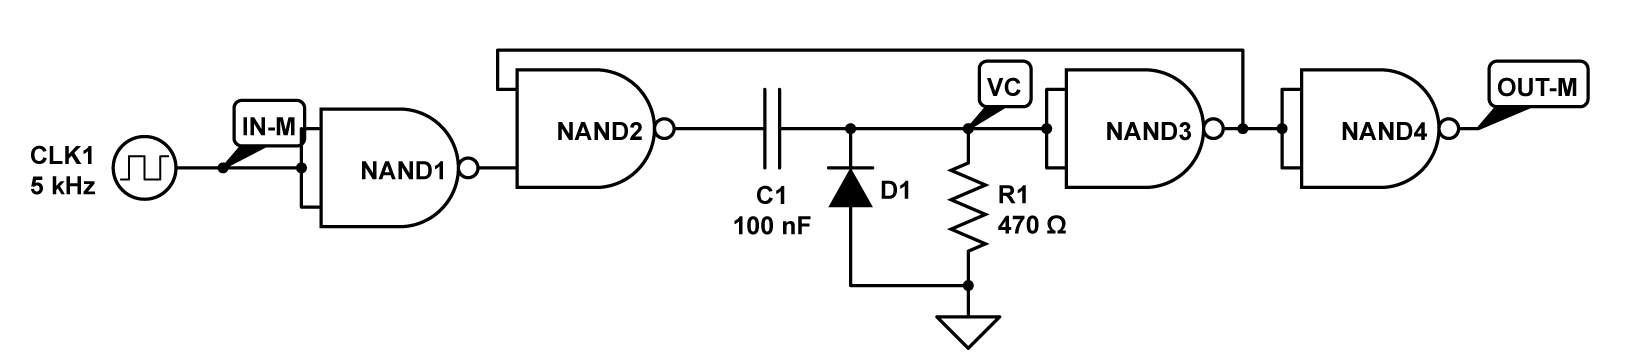
\includegraphics[scale=0.6]{monostabile.png}
	\caption{Circuito multivibratore monostabile}
	\label{f:monostabile}
\end{figure}

\begin{figure}[h]
	\centering
	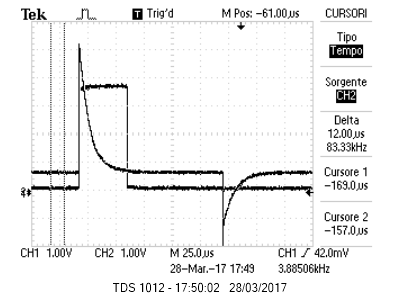
\includegraphics[scale=0.6]{monostabile_out_nand4.png}
	\caption{Ingresso IN-M del multivibratore monostabile (impulsi generati all'uscita del passa-alto), e uscita OUT-M (onda quadra) }
	\label{f:monostabile_out_nand4}
\end{figure}

\begin{figure}[h]
	\centering
	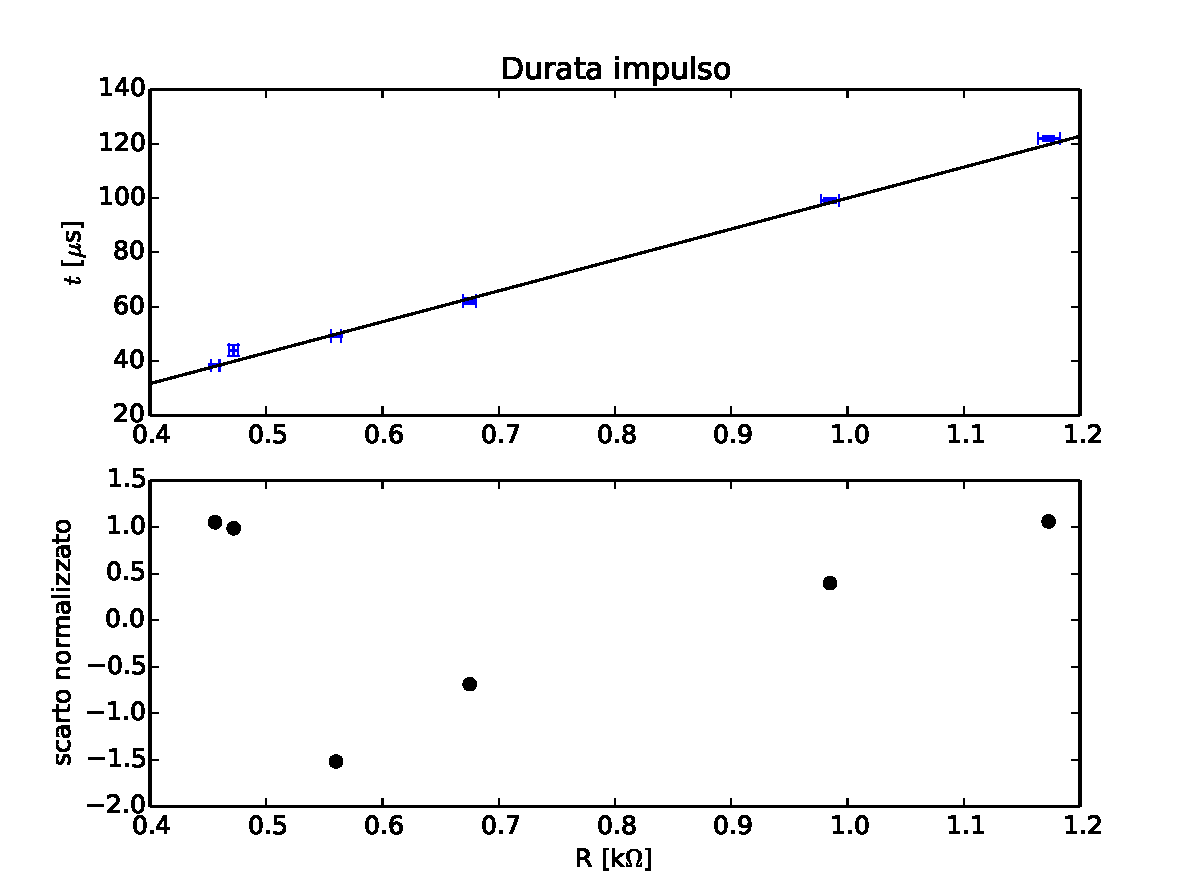
\includegraphics[scale=0.4]{impulso.pdf}
	\caption{Durata impulso in uscita OUT-M del monostabile in funzione di $R_{1}$}
	\label{f:impulso}
\end{figure}
	
\begin{figure}[h]
	\centering
	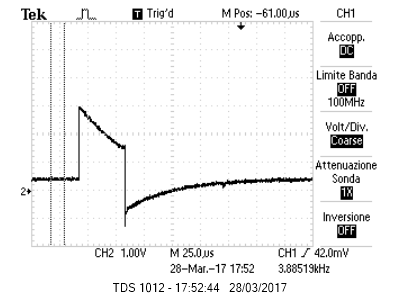
\includegraphics[scale=0.6]{monostabile_Vc.png}
	\caption{Uscita Vc del multivibratore monostabile e segnale in uscita OUT-M (l'onda quadra)}
	\label{f:monostabile_Vc}
\end{figure}

\begin{figure}[h]
	\centering
	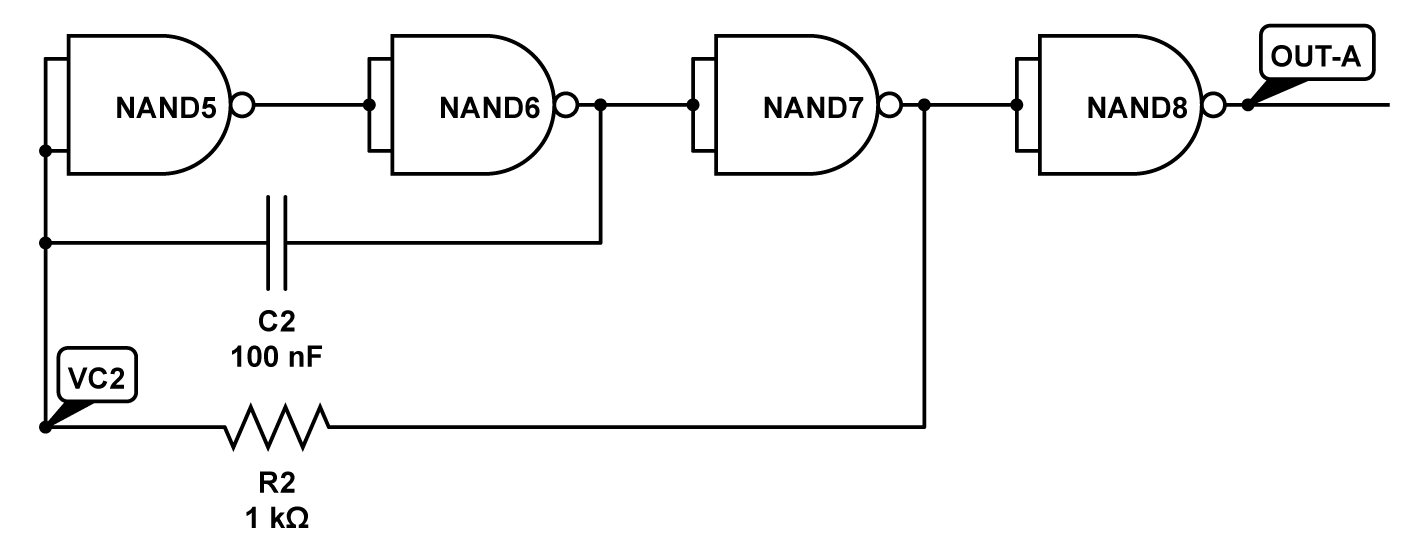
\includegraphics[scale=0.4]{astabile.png}
	\caption{Circuito multivibratore astabile}
	\label{f:astabile}
\end{figure}

\begin{figure}[h]
	\centering
	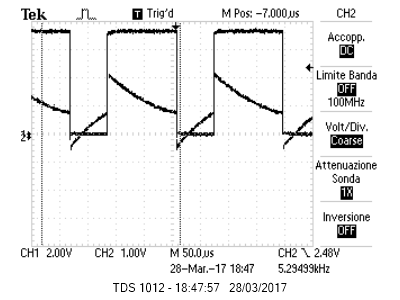
\includegraphics[scale=0.6]{out_vc.png}
	\caption{Circuito astabile,uscita OUT(onda quadra) e VC2}
	\label{f:astabile_out_vc}
\end{figure}

\begin{figure}[h]
	\centering
	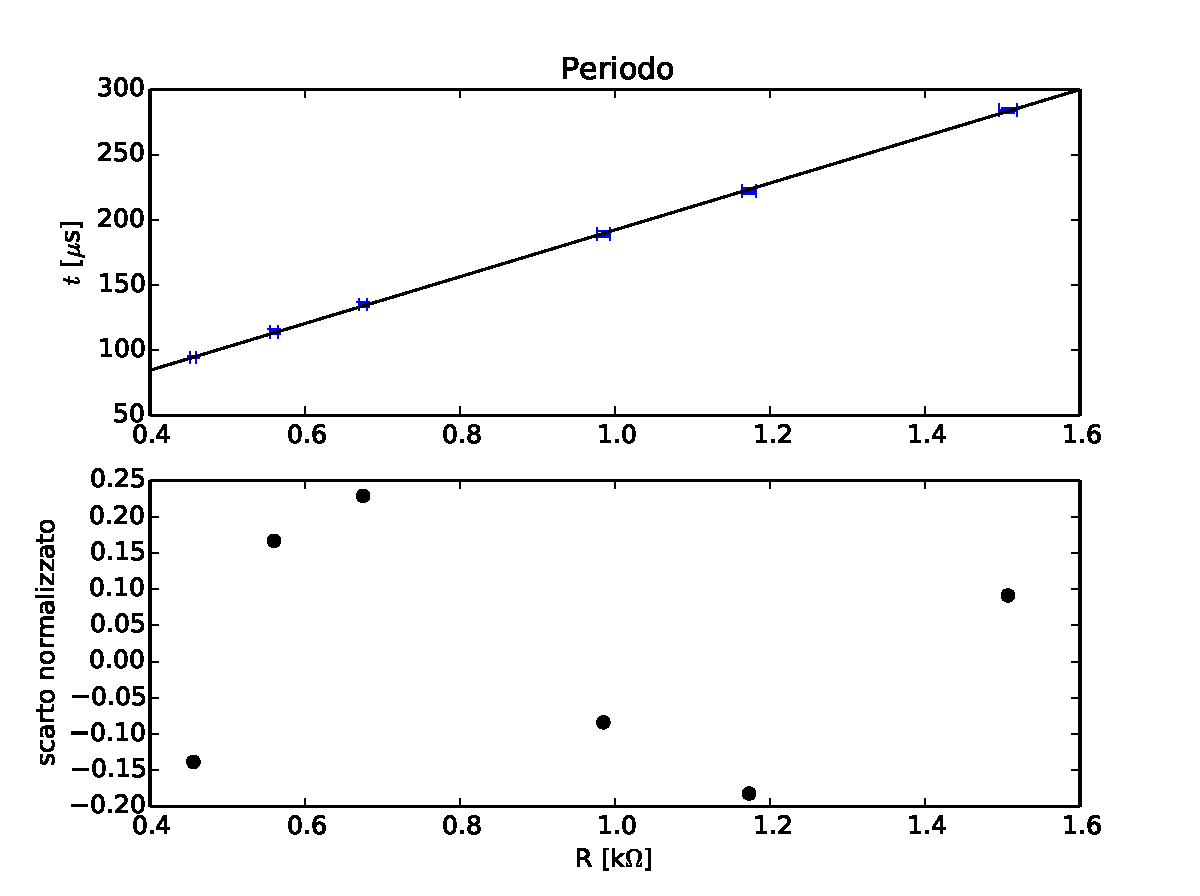
\includegraphics[scale=0.4]{periodo.pdf}
	\caption{Durata periodo in uscita OUT-A dell'astabile in funzione di $R_{2}$}
	\label{f:periodo}
\end{figure}

\begin{figure}[h]
	\centering
	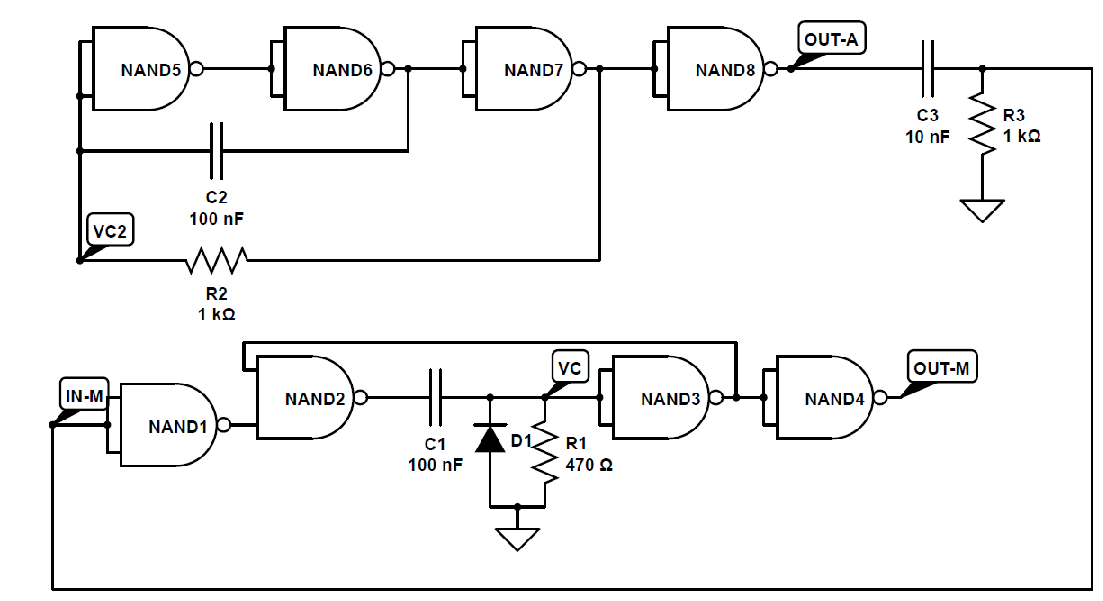
\includegraphics[scale=0.4]{generatore_circuito.png}
	\caption{Generatore di onde quadre}
	\label{f:generatore_circuito}
\end{figure}

